\documentclass{jarticle}

\usepackage{latexsym}
\usepackage{graphicx}

\title{情報科学演習及び実験1(Ocamlの基礎)}
\author{IS2 6316047 出納 光}
\begin{document}

\maketitle

\section{1. dellt}
\begin{verbatim}
# dellt;;
- : int -> ’a list -> ’a list = <fun> 
\\

\end{verbatim}

\newpage
\section{アルゴリズムの説明}
フローチャートを用いたアルゴリズムの説明。
\begin{figure}[!h]
\begin{center}
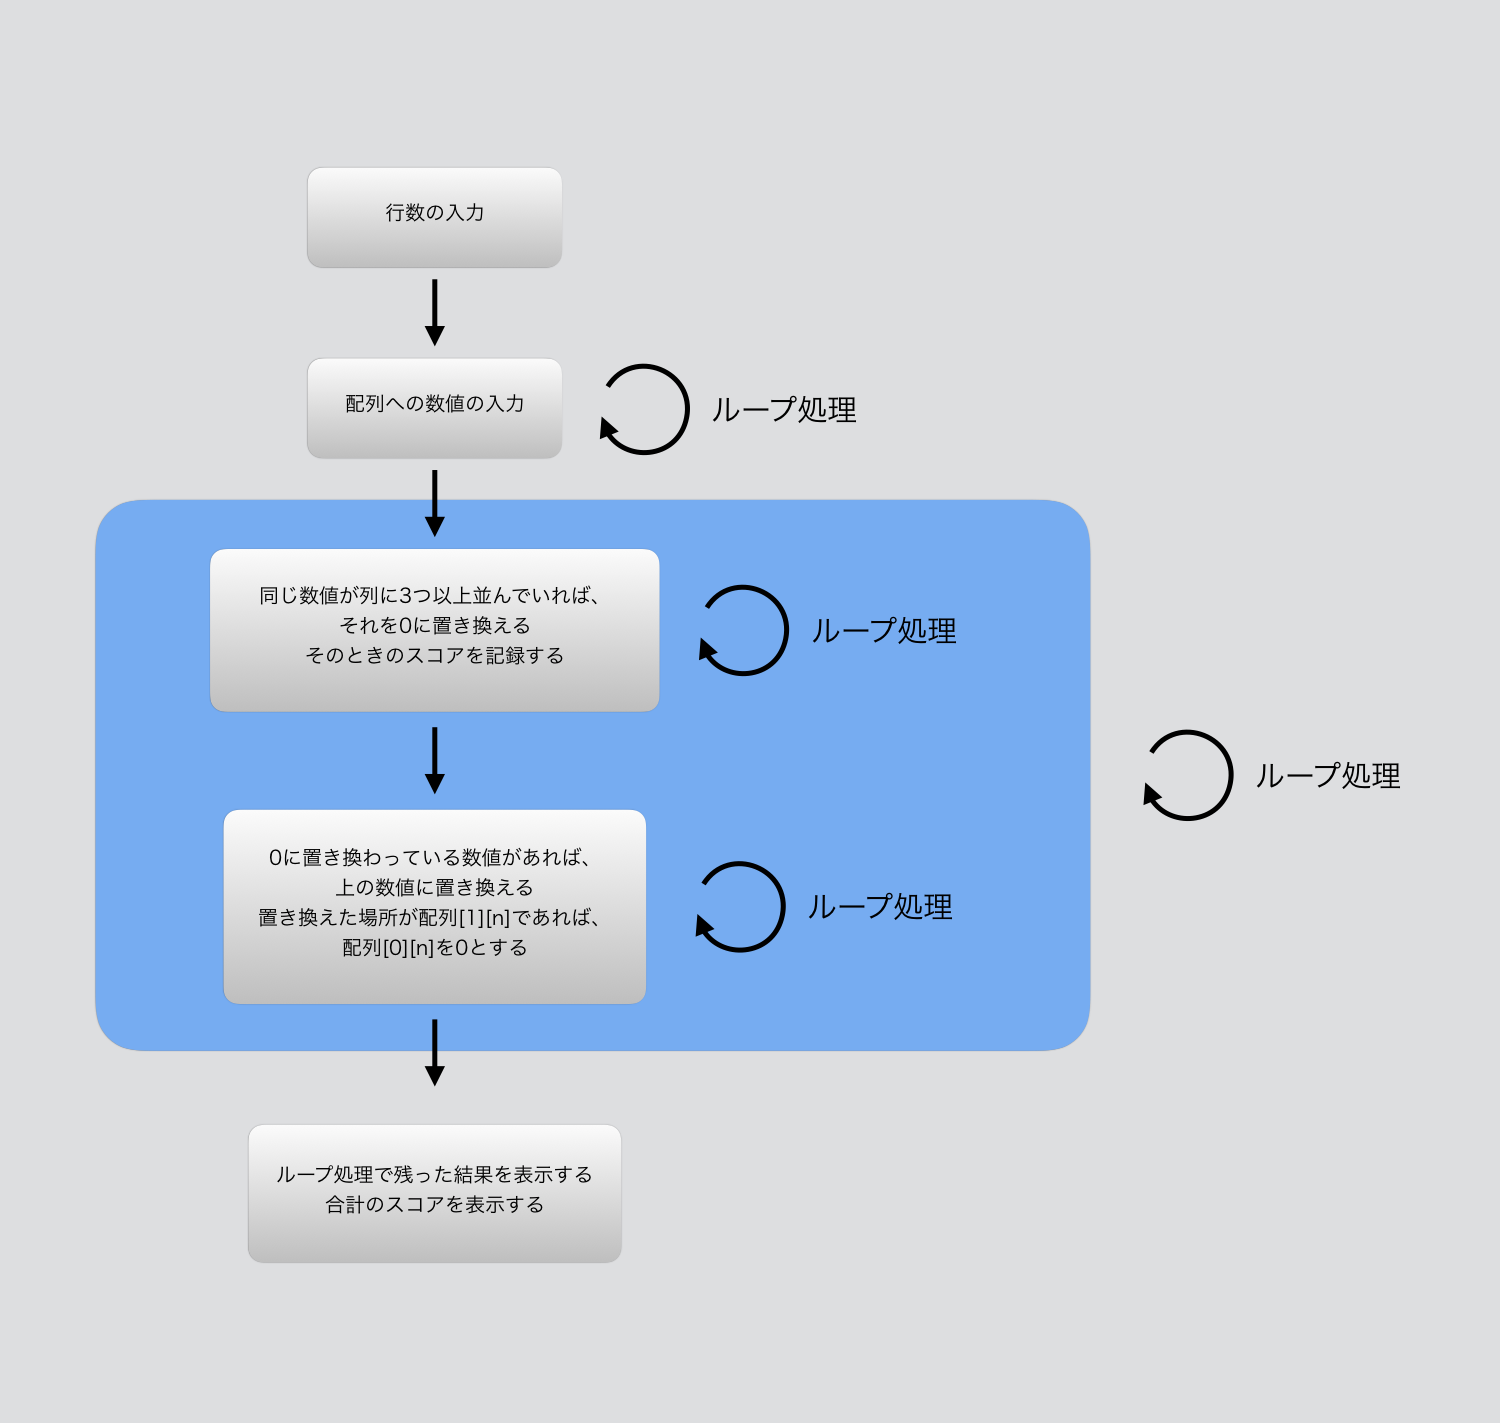
\includegraphics[scale=0.23]{c_algorithm.eps}
\end{center}
\caption{アルゴリズム}
\end{figure}

\newpage
\section{プログラムの説明}
\begin{verbatim}
1.scanfにより行数を入力する。
2.指定された行数及び5列の配列に、scanfにより数値を入力する。
3.隣り合った5つの配列が同じ数値であれば、それらの合計の数値を保存し、0に置き換える。
4.隣り合った4つの配列が同じ数値であれば、それらの合計の数値を保存し、0に置き換える。
5.隣り合った3つの配列が同じ数値であれば、それらの合計の数値を保存し、0に置き換える。
6.3-5を配列[0][0]から[0][4]、[1][0]から[1][4]と、[4][4]まで順にチェックする。
7.もし0があれば、その配列を行数が1つ上の配列の数値に置き換え、置き換え元の配列は0にする。ただし、もしそのときの行数が[1]の場合、上の配列は0にする。
8.7を一番下の行の配列から順にチェックする。ただし、これは行数分だけ繰り返し、逐次石を落としきる。
9.3-8を行数分だけ繰り返し、これ以上ないように石を消しきる。
10.記録していたスコアの合計と最終状態の配列を表示する。
\end{verbatim}

\newpage
\section{実行結果}
\begin{figure}[!h]
\begin{center}
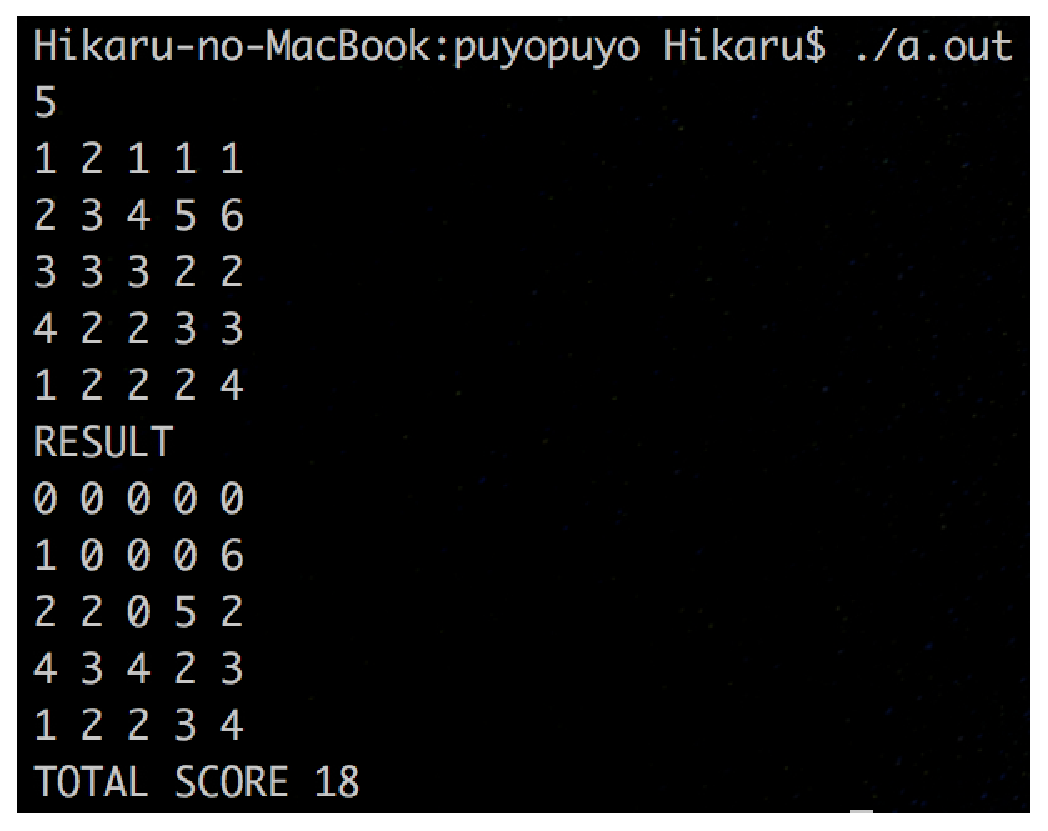
\includegraphics[scale=0.38]{c_result1.eps}
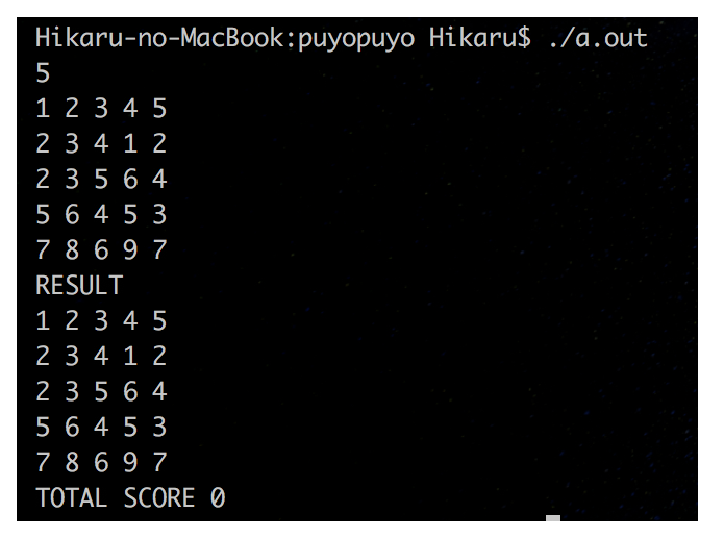
\includegraphics[scale=0.565]{c_result2.eps}
\newpage
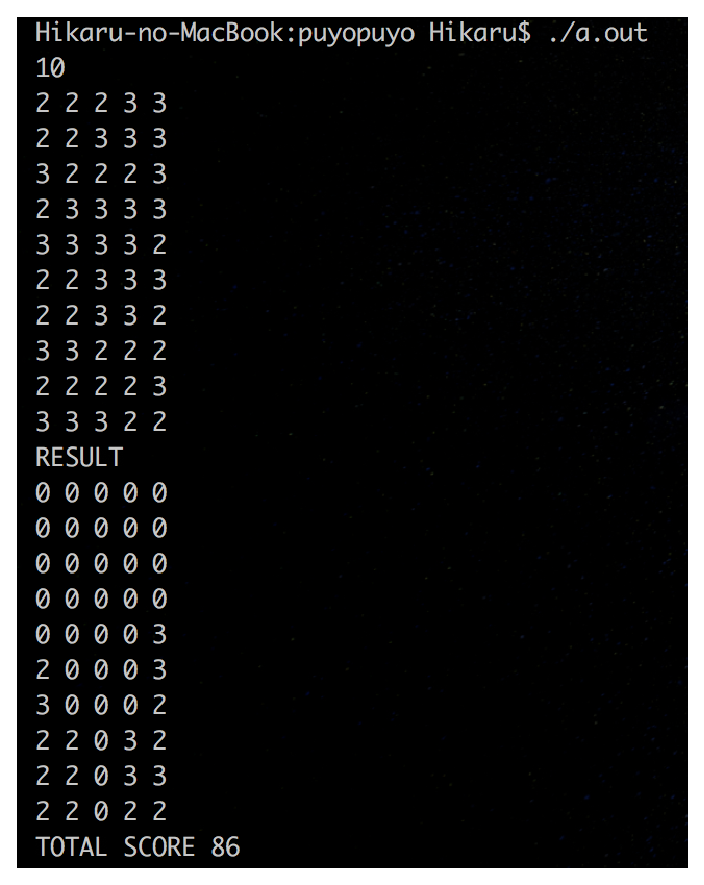
\includegraphics[scale=0.57]{c_result3.eps}
\end{center}
\caption{実行結果}
\end{figure}

\newpage
\section{考察}
\begin{verbatim}
石を下に落とす場合、0になっている石と数値の入っている石を入れ替えるやり方が可読性が高く、簡素で、速いプログラムであると思ったが、うまく入れ替えるやり方を考える時間がなかった。
\end{verbatim}

\end{document}
